\documentclass[
	aspectratio=169, % default is 43
	8pt, % font size, default is 11pt
	%handout, % handout mode without animations, comment out to add animations
	%nosectionframes, % disable automatic frames at the begin of each section (default: sectiontitleslides in beamer mode and sectionoverviews in handout mode)
	%sectiontitleslides, % enable an automatic section title slide at the begin of each section
	%sectionoverviews, % enable an automatic section overview at the begin of each section
]{beamer}

\usepackage{../beamerthemeuulm} % use the inofficial uulm beamer theme
\usepackage{tikz}
\usepackage{amsmath,amssymb}
\usepackage{xcolor}

\usepackage[ruled,linesnumbered]{algorithm2e}
\usepackage{pifont}% http://ctan.org/pkg/pifont
\newcommand{\cmark}{\ding{51}}%
\newcommand{\xmark}{\ding{55}}%
\usepackage{amsmath}
\usepackage{amsfonts}
\usepackage{amssymb}
\usepackage{tikz-qtree}
\usepackage{pgfplotstable}
\pgfplotsset{
   compat=1.16
}



\newcommand{\VarName}[1]{\textnormal{\emph{#1}}}
\usetikzlibrary{decorations.pathreplacing,calligraphy}
\setfaculty{infIngPsy} % set the color scheme for your faculty here [med/infIngPsy/math/nat]
\usetikzlibrary{positioning}
\usetikzlibrary{overlay-beamer-styles}
\usetikzlibrary{arrows.meta}

\usetikzlibrary{trees}

\tikzset{hide on/.code={\only<#1>{\color{white}}}}


%\institutelogo{sp} % set the institute logo
%\universitylogo{uulm} % set a new university logo
%\clearuniversitylogo % clear existing university logo
%\clearinstitutelogo % clear existing institute logo
%\uulmlogos{sp,uulm} % freely configure multiple logos (overwrites any other logo setting)

%\usepackage[ngerman]{babel} % use this line for slides in German

%\setmycolumnsdefault{keep} % change the default for 'mycolumns' environment (e.g., 'keep' to animate all column environments per default)

%\includeonlyframes{current} % default mechanism of beamer to include only labeled frames, can be used for debugging or drafting

\title[Projected d-DNNF Compilation]{Projected d-DNNF Compilation for Feature Models} % short title is used for the slide footer but optional
\subtitle{Master's Thesis} % subtitles are optional at all
\author[Jacob Loth]{Jacob Loth} % short author title is used for the slide footer but optional
\date{\today} % use a particular date here if needed

\begin{document}

\maketitle % title page with default picture

\section{Motivation}
\subsection{Feature Models}
\begin{frame}{\insertsubsection}
	\centering
	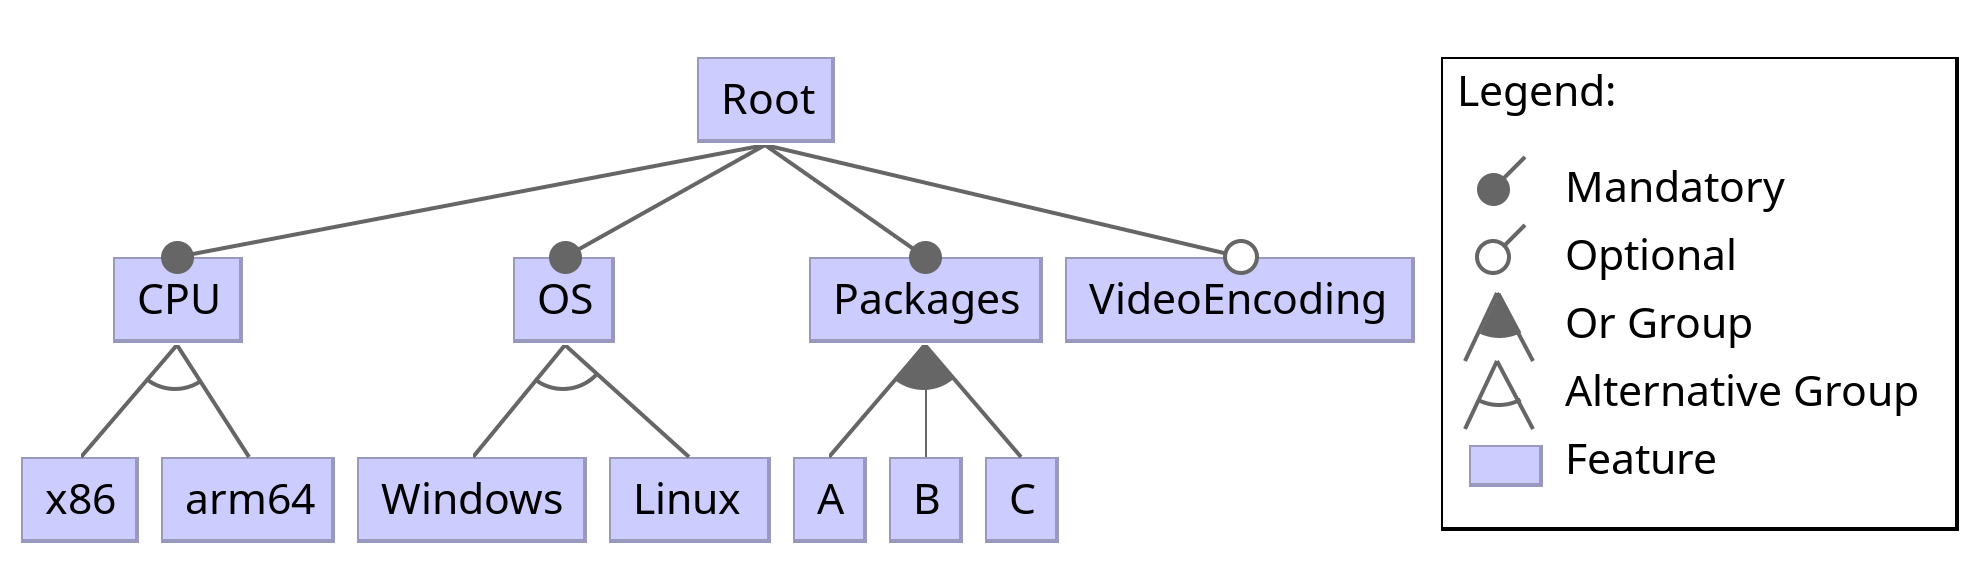
\includegraphics[width=10cm]{fm.png}
\end{frame}
\subsection{Feature-Model Slicing}
\tikzstyle{tree}=[draw=black,thick,anchor=west]
\tikzstyle{selected}=[draw=red,fill=red!30]
\tikzstyle{optional}=[dashed,fill=gray!50]
\begin{frame}{\insertsubsection}
	\begin{block}{Feature Model}
	\centering
	\begin{tikzpicture}[%
	  grow via three points={one child at (0.5,-0.7) and
	  two children at (0.5,-0.7) and (0.5,-1.4)},
	  edge from parent path={(\tikzparentnode.south) |- (\tikzchildnode.west)}]
	\node[tree](hw) {Hardware}
		child { node[tree] {arm64}}		
		child { node[tree] {x86}}
		child { node[tree] {VideoEncoding}};
	\node[tree](sw)[right = 4cm of hw] {Software}
		child { node[tree] {Windows}}	
		child { node[tree] {Linux}}			
		child { node[tree] {Packages*}};
	\draw[<->, visible on=<2->] (sw) -- (hw) node[midway,fill=white] {\emph{constraints}};
	\end{tikzpicture}
	\end{block}
	\begin{block}<3->{Problem}
		How many hardware configurations?
	\end{block}
	\begin{block}<4->{Transitive Constraints}

		\begin{tabular}[t]{cc}
			$\text{VideoEncoding} \implies \text{Windows}$&\visible<5>{  \hspace{0.5cm}$\text{Sliced: VideoEncoding} \implies \text{x84}$}\\
			$\text{Windows}\implies \text{x86}$ &
			
		\end{tabular}

	\end{block}

	

	
		
\end{frame}

\subsection{Feature-Model Counting}
\begin{frame}{\insertsubsection}
	\begin{block}{Problem}
		{\color{red} How many} hardware configurations?
	\end{block}\pause
	\centering
	\begin{tikzpicture}[]
		\node[](sharpsat){\begin{tabular}{c}
\includegraphics[width =2cm]{sharpsat.png}\\ Counts the number of solutions of a boolean formula \end{tabular}};
	\end{tikzpicture}
\end{frame}
\begin{frame}{\insertsubsection}
	\begin{block}{Problem}
		\only<1>{{\color{red} How many} hardware configurations?}
		\only<2>{ How many hardware configurations {\color{red} with arm64?}}
		\only<3->{ How many hardware configurations {\color{red} with X ?}}
	\end{block}
	\only<0->{
	\begin{tikzpicture}[]
		\node[tree](fm){Feature-Model};
		\node[tree,right= 0.5cm of fm](cnf){\begin{tabular}{c} CNF: \\ $(A \lor B \lor \neg C) \land (\neg B \lor \neg C) \dots$  \end{tabular}};
		\node[tree,tree,right= 0.5cm of cnf,visible on = <1-6>](slice){\begin{tabular}{c} Slice:\\$(A \lor B)\land (\neg B)\dots$\end{tabular}};
		\node[right= 1.0cm of slice,visible on=<1-3>](sharpsat){
\includegraphics[width =1cm]{sharpsat.png}};
		\node[below= 0.5cm of sharpsat,visible on=<2-3>](sharpsat1){
\includegraphics[width =1cm]{sharpsat.png}};
		\node[above= 0.5cm of sharpsat,visible on=<3-3>](sharpsatN){$...$};
		\node[right= 1.0cm of slice,visible on=<4-6>](ddnnf){
\includegraphics[width =2cm,height=2cm]{ddnnf.png}};
		\node[above= 0.5cm of ddnnf,visible on=<5-6>,draw=black,thick](queries){\begin{tabular}{l} Counting Queries:\\arm64=true\\ $\dots$ \end{tabular} };
		\node[right= 1.0cm of cnf,visible on=<7>](pddnnf){
\includegraphics[width =2.7cm]{pdnnf.png}};
		\node[above= 0.5cm of pddnnf,visible on=<7>,draw=black,thick](queries1){\begin{tabular}{l} Counting Queries:\\arm64=true\\ $\dots$ \end{tabular} };
		\draw[->] (fm)--(cnf);
		\draw[->,visible on = <1-6>] (cnf)--(slice);
		\draw[->,visible on = <1-6>] (slice)--(sharpsat);
		\draw[->,visible on=<2-3>] (slice.east)--(sharpsat1) node[near end,left] {arm64=true};
		\draw[->,visible on=<3-3>] (slice.east)--(sharpsatN);
		\draw[->,visible on=<5-6>] (queries)--(ddnnf);
		\draw[->,visible on=<5-6>] (queries)--(ddnnf);
		\draw[->,visible on=<7>] (cnf)--(pddnnf);
		\draw[->,visible on=<7>] (queries1)--(pddnnf);
		\draw [decorate,
    decoration = {brace},thick,red,visible on = <6>] (11,-0.75) --  (7.3,-0.75) node[midway,below] {can be slow};
	\end{tikzpicture}}
\end{frame}
\subsection{Projected d-DNNF Compilation}
\begin{frame}{\insertsubsection}
	\centering
\begin{tikzpicture}[]
	\node[right= 1.0cm of cnf](pddnnf){\begin{tabular}{c} 
\includegraphics[width =2.7cm]{pdnnf.png} \\ Compiles $F$ into d-DNNF while slicing a set of variables $Y$ and keep a set of projected variables $X$  \end{tabular}};
\end{tikzpicture}
\pause
\begin{block}{Related Problem}
	Projected Model Counting(PMC):\\
	$\implies$Counting all assignments to variables $Var(F)-Y$ that have some extension to a solution in $F$\\
\end{block}
\end{frame}
\subsection{What are d-DNNFs?}
\begin{frame}{\insertsubsection}
	\begin{columns}[T]
		\begin{column}{.34\textwidth}
	\begin{block}{Any boolean formula that has...}
		\begin{itemize}
			\item<2-> Decomposable AND-Nodes
			\item<4-> Deterministic OR-Nodes (If-Then-Else)
			\item<6-> Negations only right before variables
		\end{itemize}
	
	\end{block}
	\begin{block}<8>{d-DNNF Compilation:}
		Turn CNF into d-DNNF
	\end{block}
\end{column}
\begin{column}{.5\textwidth}
	\begin{block}{}
	\begingroup
    \fontsize{12pt}{12pt}\selectfont
	
	\only<2-3>{ \begin{align*}
		(A \lor B) \land (A \lor C) \implies \text{Not Decomposable {\color{red} \xmark}}\\
		\visible<3>{(A \lor B) \land (D \lor C) \implies \text{Decomposable {\color{green} \checkmark}}}
	\end{align*}}
	\only<4-5>{ \begin{align*}
		(A \lor A) \implies \text{Not Deterministic {\color{red} \xmark}}\\
		\visible<5>{ (A \land B) \lor (A \land \neg B) \implies \text{Deterministic  {\color{green} \checkmark}}}
	\end{align*}}
	\only<7-8>{
		\begin{tabular}{c}	
		Knowledge Compilation\\
		+\\
		Linear Time Model Counting
		\end{tabular}
	}
	\endgroup
	\end{block}
\end{column}
\end{columns}
\end{frame}
\subsection{d-DNNF Compilation}

\begin{frame}{\insertsubsection}
	\begin{columns}[c]
		\begin{column}{.5\textwidth}
	\centering
	\begin{block}{DPLL}
	\begin{overlayarea}{10cm}{4.44cm}
		

		

	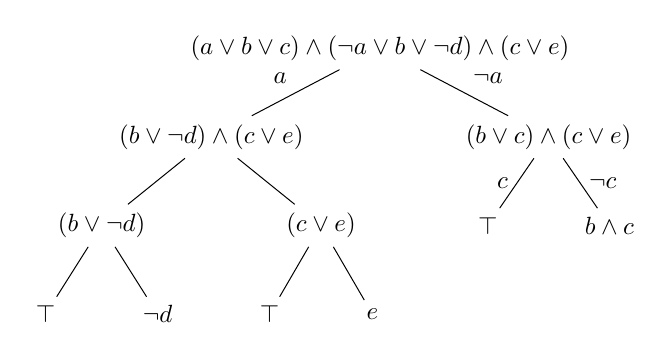
\begin{tikzpicture}[every tree node/.style={},
	level distance=1.25cm,sibling distance=1cm,
	scale=0.9,
	edge from parent path={(\tikzparentnode) -- (\tikzchildnode)}]
 \Tree
 [. \node[visible on=<1->]{$(a \lor b \lor c) \land (\neg a \lor b  \lor \neg d ) \land (c \lor e)$};
	 \edge[visible on=<2->] node[auto=right] {$a$};
	 [. \node[visible on=<2->]{$( b  \lor \neg d ) \land (c \lor e)$ };
	 	\edge[visible on=<4->] node[auto=right] {$$};
	 	[. \node[visible on=<4->]{$(b \lor \neg d)$} ;
		 	\edge[visible on=<5->] node[auto=right] {$$};
	 		[.\node[visible on=<5->] {$\top$};  ] 
			\edge[visible on=<5->] node[auto=right] {$$};
	 		[.\node[visible on=<5->]{$\neg d$};  ] 
	 	]
		\edge[visible on=<4->] node[auto=right] {$$};
	 	[.\node[visible on=<4->]{$(c \lor e)$};
		 	\edge[visible on=<6->] node[auto=right] {$$};
	 		[.\node[visible on=<6->]{$\top$};  ]
			 \edge[visible on=<6->] node[auto=right] {$$};
			[.\node[visible on=<6->]{$e$};  ] 
	]
	]
	 \edge[visible on=<3->] node[auto=left] {$\neg a$};
	 [.\node[visible on=<3->]{$(b \lor c) \land (c \lor e)$};
		 \edge[visible on=<7->] node[midway,left] {$c$};
		 [.\node[visible on=<7->]{$\top$};  ]
		 \edge[visible on=<7->] node[midway,right] {$\neg c$};
		 [.\node[visible on=<7->]{$b \land c$};  ]
	]
 ]
 \end{tikzpicture}
\end{overlayarea}


\end{block}
\end{column}
\begin{column}{.5\textwidth}
	\begin{block}<8>{DNNF}
		
	\centering
	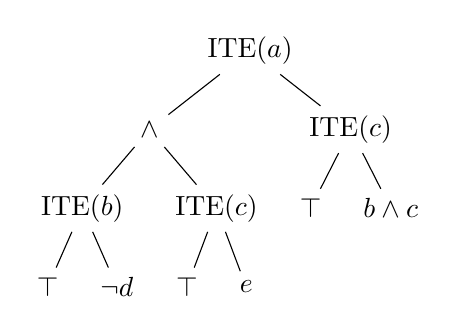
\begin{tikzpicture}[every tree node/.style={},
		level distance=1cm,sibling distance=0.3cm,
		scale=1.,
		edge from parent path={(\tikzparentnode) -- (\tikzchildnode)}]
	 \Tree
	 [.{$\text{ITE}(a)$}
		 [.{$\land$ }
		 [.{$\text{ITE}(b)$}  
		 [.{$\top$}  ] 
		 [.{$\neg d$}  ] 
		 ]
		 [.{$\text{ITE}(c)$}  
			 [.{$\top$}  ] 
			[.{$e$}  ] 
		]
		]
		 [.{$\text{ITE}(c)$} 
			 [.{$\top$}  ]
			 [.{$b \land c$}  ]
		]
	 ]
	 \end{tikzpicture}
	
	\end{block}
	\begin{block}<8>{}
		\hspace{1cm} ITE = If Then Else
	\end{block}

	

\end{column}
\end{columns}





\end{frame}
\section{Our Contributions (so far)}
\subsection{Projected d-DNNF Compilation}
\begin{frame}[fragile]{\insertsubsection}
	\begin{block}{Concept}
	Projected variables = $a,b,d$\\
	Sliced variables = $c,e$
	\end{block}
	
	\begin{block}{}
		\centering
		\begin{overlayarea}{10cm}{4.44cm}
\begin{tikzpicture}[every tree node/.style={},
	level distance=1.25cm,sibling distance=1cm,
	scale=0.9,
	edge from parent path={(\tikzparentnode) -- (\tikzchildnode)}]
 \Tree
 [. \node[visible on=<1->]{$(a \lor b \lor c) \land (\neg a \lor b  \lor \neg d ) \land (c \lor e)$};
	 \edge[visible on=<2->] node[auto=right] {$a$};
	 [. \node[visible on=<2->]{$( b  \lor \neg d ) \land (c \lor e)$ };
	 	\edge[visible on=<4->] node[auto=right] {$$};
	 	[. \node[visible on=<4->]{$(b \lor \neg d)$} ;
		 	\edge[visible on=<5->] node[auto=right] {$$};
	 		[.\node[visible on=<5->] {$\top$};  ] 
			\edge[visible on=<5->] node[auto=right] {$$};
	 		[.\node[visible on=<5->]{$\neg d$};  ] 
	 	]
		\edge[visible on=<4->] node[auto=right] {$$};
	 	[.\node[visible on=<4->]{\only<4-5>{$(c \lor e)$} \only<6->{\color{red} $\top$}  };]
	]
	 \edge[visible on=<3->] node[auto=left] {$\neg a$};
	 [.\node[visible on=<3->]{$(b \lor c) \land (c \lor e)$};
		 \edge[visible on=<7->] node[midway,left] {$b$};
		 [.\node[visible on=<7->]{$\top$};  ]
		 \edge[visible on=<7->] node[midway,right] {$\neg b$};
		 [.\node[visible on=<7->]{  \only<7>{ $(c \lor e)$ } \only<8->{\color{red} $\top$}   };  ]
	]
 ]
 \end{tikzpicture}

\end{overlayarea}
\end{block}


\end{frame}
\subsection{Projected d-DNNF Compilation}
\begin{frame}{\insertsubsection}
	\begin{block}{Implementation}
		Based on the D4 d-DNNF compiler
		\begin{itemize}
			\item Replace sets of clauses containing only projected variables with $\top$ or $\bot$ 
			\item Always ignore sliced literals
			\item Restrict variable selection to projected set \pause $\implies$ losing D4s variable selection heuristics
		\end{itemize}
	\end{block}
\end{frame}
\subsection{Optimizations}
\begin{frame}{\insertsubsection}
	\begin{block}{Variable Selection}
		Crucial for performance: Separate clauses to generate decomposable AND-Nodes\\
		\vspace{0.25cm}
		\begin{center}
			
	
		\only<2>{
		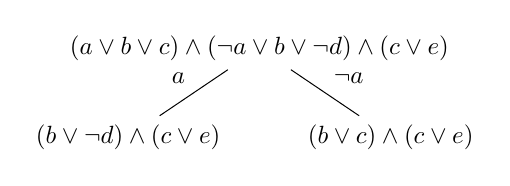
\begin{tikzpicture}[every tree node/.style={},
			level distance=1.25cm,sibling distance=1cm,
			scale=0.9,
			edge from parent path={(\tikzparentnode) -- (\tikzchildnode)}]
		 \Tree
		 [. \node {$(a \lor b \lor c) \land (\neg a \lor b  \lor \neg d ) \land (c \lor e)$};
			\edge node[auto=right] {$a$};
			[. \node[]{$( b  \lor \neg d ) \land (c \lor e)$ };]
			 \edge node[auto=left] {$\neg a$};
			[. \node{$(b \lor c) \land (c \lor e)$};]
		]
		\end{tikzpicture}}

		\only<3->{
			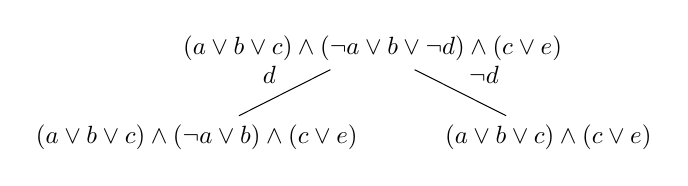
\begin{tikzpicture}[every tree node/.style={},
				level distance=1.25cm,sibling distance=1cm,
				scale=0.9,
				edge from parent path={(\tikzparentnode) -- (\tikzchildnode)}]
			 \Tree
			 [. \node {$(a \lor b \lor c) \land (\neg a \lor b  \lor \neg d ) \land (c \lor e)$};
				\edge node[auto=right] {$d$};
				[. \node[]{$(a \lor b \lor c) \land (\neg a \lor b ) \land (c \lor e)$ };]
				 \edge node[auto=left] {$\neg d$};
				[. \node{$(a \lor b \lor c) \land (c \lor e) $};]
			]
			\end{tikzpicture}}
		\end{center}
		\only<4->{D4 separates clauses using cut sets, \emph{BUT} cuts may contain sliced variables\\ 
			$\implies$ Adapt D4s variable selection heuristics to favor clean cuts}
	\end{block}
	\begin{block}<5->{Preprocessing}
		Make the problem smaller, various methods adapted from PMC\\
		Problem: preserve true equivalence
	\end{block}
	\begin{block}<6->{Technical Stuff}
		Cache and branch friendly variable and clause renaming/ordering
	\end{block}
\end{frame}
\subsection{Results}
\begin{frame}{\insertsubsection}
	\centering
	\begin{tikzpicture}[]
		\begin{axis}[legend pos=north west,width=10cm,height=5cm,scale only axis,ylabel={time(s)},xlabel={\#solved}]
			\addplot[black,mark=x] table {base.csv};
			\addlegendentry{ours initial}
			\addplot[green,mark=x] table {proj_d4.csv};
			\addlegendentry{ours current}
			\addplot[red,mark=x] table {slice_d4.csv};
			\addlegendentry{slice}
			\addplot[blue,mark=x] table {gpmc.csv};
			\addlegendentry{gpmc}
		\end{axis}
	\end{tikzpicture}
\end{frame}
\subsection{Current State}
\begin{frame}{\insertsubsection}
	\begin{tabular}{ll}
		Concept: & Done \\
		Implementation: & Done\\
		Explore optimization: & Almost Done (preprocessing, fine-tuning)  \\
		Evaluation: & WIP (more tests needed) \\
		Writing the thesis: & Started \\
	\end{tabular}
\end{frame}
\subsection{The End}
\begin{frame}{\insertsubsection}
\end{frame}
\subsection{Projected d-DNNF Compilation}
\begin{frame}{\insertsubsection}
	\centering
\begin{tikzpicture}[]
	\node[right= 1.0cm of cnf](pddnnf){\begin{tabular}{c} 
\includegraphics[width =2.7cm]{pdnnf.png} \\ Compiles $F$ into d-DNNF while slicing a set of variables $Y$ and keep a set of projected variables $X$  \end{tabular}};
\end{tikzpicture}

\end{frame}







\end{document}